\documentclass[nochap]{apuntesURJC}





\title{Historia de la criptografía}
\author{Víctor de Juan, Gustavo Martínez, Cristina Martínez y Virginia Vadillo}
\date{16/17 C1}


\begin{abstract}

A lo largo de este trabajo realizaremos un recorrido por la historia de la criptografía centrándonos en el punto de vista de los ``países occidentales'' en que habitamos.

Empezaremos describiendo qué es las criptografía y cuál es su motivación, lo que nos permitirá entender cuándo surgió, en qué momento vivió un mayor desarrollo y cómo ha evolucionado a lo largo del tiempo.

Para cada civilización o momento histórico del que hablemos veremos una pequeña descripción del contexto histórico en el que se desarrollan los criptosistemas que estudiaremos, seguido de una descripción de los mismos. También analizaremos su funcionamiento y los ataques contra ellos desde una perspectiva matemática.

\end{abstract}

\begin{document}


\maketitle % Print the title/author/date block

\setcounter{tocdepth}{3} % Set the depth of the table of contents to show sections and subsections only

\tableofcontents % Print the table of contents
\newpage

%\listoffigures % Print the list of figures

%\listoftables % Print the list of tables


%----------------------------------------------------------------------------------------
%	INTRODUCTION
%----------------------------------------------------------------------------------------

%\cite{Figueredo:2009dg}.
% http://www.studentpulse.com/articles/41/a-brief-history-of-cryptography

\section{Introducción}
Las primeras formas de criptografía consistían en la escritura de mensajes que la mayoría de la gente no fuese capaz de leer. De hecho, la palabra criptografía procede de las palabras griegas ``kryptos'' y ``graphien'', que significan ``oculto'' y ``escritura'' respectivamente.

La necesidad de mantener comunicaciones privadas ha estado ligada al ser humano desde este que salió de las cavernas y empezó a vivir en sociedad.

Tan pronto como aparecieron diferentes grupos de homínidos, surgió la rivalidad entre estos y con ella, la necesidad de mantener comunicaciones al margen del enemigo.

Aunque estos grupos de homínidos ya estaban presentes en el Paleolítico, y con ellos las rivalidades que acabamos de comentar, no tiene sentido hablar de la criptografía como tal hasta la aparición de la escritura.\\


Originalmente la criptografía tenía como objetivo convertir un mensaje en una secuencia de símbolos ilegibles a fin de proteger el contenido del mensaje durante el tiempo en que este era transportado desde el emisor al receptor. En la actualidad, en cambio, los objetivos de la criptografía han evolucionado. Desde la simple misión de mantener la confidencialidad hemos avanzado hasta a un desarrollo de la criptografía que permite garantizar, entre otros aspectos, la integridad del mensaje y la autenticación tanto del emisor como del receptor.

Un concepto \textbf{fundamental} en la concepción de la criptografía es que la seguridad\footnote{El concepto de seguridad engloba todas las propiedades que se esperan de un criptosistema como son confidencialidad, integridad y autenticación.} no puede basarse en la ocultación del mensaje. Se asume que el enemigo será capaz de interceptar algún mensaje y se trata de garantizar que no será capaz de comprenderlo.\\

La evolución de la criptografía se basa en tres pasos fundamentales que se repiten una y otra vez a lo largo de la historia:
\begin{enumerate}
\item Alguien idea un \textbf{procedimiento nuevo} que permite cifrar mensajes y garantizar que estos sólo puedan ser descifrados e interpretados por su destinatario, creando así un \textbf{criptosistema}.

\item En un momento de necesidad, generalmente en períodos de guerra, comienza a utilizarse este \textbf{criptosistema} para mantener comunicaciones entre aliados que el enemigo no pueda comprender.

\item El enemigo (\textbf{atacante}, como suele decirse en el ámbito de la criptografía) estudia el \textbf{criptosistema} y desarrolla los métodos e instrumentos necesarios para poder descifrar un mensaje interceptado.

\item Se encuentra una forma eficaz de descifrar mensajes con lo que el \textbf{criptosistema} queda obsoleto y hay que volver al primer paso.
\end{enumerate}

A medida que avanzan la tecnología y los conocimientos matemáticos, las herramientas de las que se dispone para descifrar mensajes son más complejas y avanzadas lo que exige el desarrollo de nuevos y mejores \textbf{criptosistemas}, entrando así en una carrera ``infinita'' en la que los \textbf{criptosistemas} han de estar siempre un paso por delante de las técnicas de descifrado.\\

\section{Edad Antigua}

La Edad Antigua comprende el período comprendido entre el final de la Prehistoria y el comienzo de la Edad Media. Este período abarca unos 5000 años, comenzando con el desarrollo de la escritura cuneiforme y finalizando con la caída del Imperio Romano de Oriente, en el año 476 d.C.

\subsection{Egipto}
El uso \textbf{más antiguo conocido} de la criptografía se encuentra en los \textbf{jeroglíficos} grabados en monumentos del Antiguo Egipto hace más de 4500 años.

La palabra \textbf{jeroglífico} proviene de la palabra griega ιερoγλvφoç, compuesta a su vez por las raíces griegas ιερoç (hierós, que significa ``sagrado'') y γλ$\upsilon$φειν(glýpheιn, que significa ``grabar''). Fue empleada por primera vez en la escrituras de Diorus Scilus (primer siglo antes de Cristo).

La \textbf{escritura jeroglífica} es un sistema de escritura caracterizado por el empleo de dibujos en lugar de simples caracteres, se trata de un sistema \textbf{ideográfico}.

La cultura egipcia surgió en el año 3.500 a.C. estableciendo su capital en Memphis. El periodo antiguo contó con 20 dinastías que se alargaron hasta el 1.100 a.C.

Esta cultura se caracterizaba por una clara división de la sociedad en diferentes estamentos: Faraón, escribas, campesinos libres y comerciantes, pueblo llano y esclavos.

Gran parte del conocimiento que tenemos acerca de este pueblo se debe al descubrimiento, por parte del imperio Napoleónico en 1799, de La Piedra Roseta, que estaba escrita en tres lenguas distintas: jeroglífico, demótico y griego (por la influencia de Alejandría). Gracias a ella pudieron comprenderse los \textbf{jeroglíficos}, cuyo significado permaneció oculto a los ojos de occidente hasta ese momento.


Desde mediados del tercer milenio a.C. y más frecuentemente en el período conocido como \textbf{Nuevo Reino} (desde 1539 hasta 1075 a.C.) los jeroglíficos adquieren una extraña apariencia. La ausencia de grupos de palabras familiares y la presencia de signos ajenos a los cánones caracterizan estos textos como textos codificados.

No obstante, no son considerados como un auténtico criptosistema (con la definición de hoy día) pues no se cree que tuvieran por objetivo el mantener comunicaciones secretas. En su lugar, se cree que fueron empleados para generar misterio e intriga entre sus lectores.

\subsection{Mesopotamia}
La región de Oriente Medio situada entre los ríos Tigris y Éufrates, en el actual estado de Irak, fue cuna de una de las primeras (cadenas de) civilizaciones de las que tenemos constancia. Fue llamada Mεσoπoταμía (Mesopotamia) en la Época Clásica cuyo significado es ``entre ríos''.

En \textbf{Mesopotamia} la primitiva estructura de aldeas evolucionó hasta ciudades estado y luego hacia imperios enormes que contenían a multitud de pueblos.

No fue hasta el siglo XIX cuando los arqueólogos comenzaron a interesarte por este territorio y se llevaron a cabo las primeras excavaciones. Allí se encontraon mosaicos, frescos e incluso tablillas de barro que contenían incisiones con un punzón, \textbf{la escritura cuneiforme}.

De entre estas tablillas, cabe destacar la famosa \textbf{tablilla Plimton}, que contiene problemas matemáticos. No hay que olvidar la tabla encontrada en al año 1500 a.C. que contiene la receta cifrada para la elaboración de un esmalte de cerámica artesanal que, al parecer, tenía una gran valor comercial.

\subsection{Grecia}
Originalmente, el territorio conocido actualmente como Grecia estaba ocupado por una serie de pueblos del Mediterráneo como los Minoicos y los Micenos. Estos pueblos fueron invadidos y derrotados por los pueblos helenos (Dorios, Jonios y Eolios) procedentes del centro de Europa.

Durante esta época, la población de Grecia se multiplicó y dio comienzo la colonización de la costa jónica.

A lo largo de su historia, Grecia nunca estuvo unida como nación sino que estaba formada por una serie de pequeñas \textbf{Ciudades Estado} que combatían entre si de manera constante formando pequeñas alianzas en ciertas ocasiones que no acostumbran a ser duraderas.

En este ambiente de guerra constante entre pueblos hermanos, era muy frecuente que un pueblo capturase a un mensajero del rival, lo que le permitiría interceptar la comunicación, conociendo así las intenciones del pueblo enemigo. Esto dio lugar a la necesidad de desarrollar un \textbf{criptosistema} que permitiera a dos personas comunicarse a distancia sin riesgo de que el mensaje sea comprendido por los enemigos.

Así surgió uno de los primeros sistemas de cifrado, propiamente dicho, conocidos. Este \textbf{criptosistema} se basaba en el uso de una \textbf{escítala}. Una \textbf{escítala} está formada por dos varas del mismo grosor, siendo este variable, y una tira de cuero o papiro. Cada participante en la comunicación se quedaba con una de las baras. La forma de comunicación consistía en enrollar la cinta en torno a la bara y escribir sobre ella longitudinalmente. El receptor del mensaje no tenía más que enrollar la cinta en su propia barra y leer longitudinalmente para poder entender el mensaje.

Si un atacante se hacía con la cinta, mientras no conociera el grosor de la barra (suponiendo que conociese el sistema empleado), no sería capaz de descifrar el mensaje.

El historiador Herodoto cuenta que en ocasiones los mensajes secretos eran escondidos, por ejemplo, tatuándolos en la cabeza de un esclavo que era enviado al destinatario una vez le hubiese crecido el pelo de nuevo. No obstante, esto no puede considerarse criptografía propiamente dicho como ya se explica en la introducción de este trabajo.

\subsubsection{Modelización actual del cifrado con Escítala}
Sistemas como este son hoy en día conocidos como sistemas de transposición. En ellos el cifrado consiste en alterar el orden de los elementos de un mensaje, sin añadir ni eliminar ningún elemento.

El proceso de cifrado con \textbf{escítala} es equivalente a disponer en una tabla cada uno de los elementos en filas y luego tomarlos en columnas, siendo el ancho de la fila el número de caras que presenta la escítala y el número de filas el resultante de dividir el largo total del mensaje entre el ancho de la fila.

\begin{minipage}{0.65\textwidth}
La tabla de la derecha muestra cómo el mensaje original:
\begin{center}
``En un lugar de la Mancha, de cuyo nombre no quiero acordarme''
\end{center}
se transforma en
\begin{center}
``Ernu  n cyna dhoocuea  on ,nqr l oudladmiau ebergM rrmaaceoe''
\end{center}
que resulta imposible de comprender si no se conoce el método de descifrado.

\end{minipage}
\begin{minipage}{0.3\textwidth}

\end{minipage}
\begin{minipage}{0.30\textwidth}
\begin{center}
\begin{tabular}{|c|c|c|c|c|c|}
\hline
E & r & n & u &   &   \\
\hline
n &   & c & y & n & a \\
\hline
  & d & h & o & o & c \\
\hline
u & e & a &   &   & o \\
\hline
n &   & , & n & q & r \\
\hline
  & l &   & o & u & d \\
\hline
l & a & d & m & i & a \\
\hline
u &   & e & b & e & r \\
\hline
g & M &   & r & r & m \\
\hline
a & a & c & e & o & e \\
\hline
\end{tabular}
\end{center}
\end{minipage}

\subsection{Roma}
\subsubsection{Entre la historia y la leyenda}
La historia de los orígenes de Roma se pierde entre las brumas de la leyenda. Sus humildes comienzos no debieron distinguirse mucho de los de tantas ciudades de la región del Lacio. Pero con el tiempo, los antiguos historiadores romanos pensaron que la ciudad escogida por los dioses para convertirse en dueña del mundo debía tener un origen heroico, que adornaron con infinidad de leyendas, muchas veces contradictorias entre sí, llenas de dioses y héroes mitológicos.

De hecho, para los modernos investigadores resulta difícil distinguir leyenda y realidad, porque a veces, inesperados descubrimientos arqueológicos sacan a la luz las huellas de personajes y sucesos que parecían meras invenciones legendarias.

Roma fue fundada, según la tradición, por dos hermanos gemelos, Rómulo y Remo, que, acompañados de bandidos y vagabundos expulsados de sus propias ciudades, decidieron fundar un nuevo asentamiento junto al Tíber. Sin embargo, los dos hermanos no se ponían de acuerdo acerca del lugar en que levantarían su ciudad. Remo prefería el promontorio del Aventino, mientras que Rómulo se inclinaba por la colina del Palatino. Así las cosas, decidieron dejar su disputa al arbitrio de los dioses y -apostados cada uno en su colina-, se quedaron esperando una señal de lo alto.

La mañana del 21 de abril del año 753 a.C., Remo contemplaba el limpio cielo primaveral desde la cima del Aventino cuando divisó seis enormes buitres sobre su colina. Lleno de euforia, echó a correr hacia Rómulo, para anunciarle su victoria. Sin embargo, en ese mismo instante, una bandada de doce pájaros sobrevolaba el Palatino. Seguro de su victoria, y sin esperar la llegada de su hermano, Rómulo cogió un arado y comenzó a cavar el pomerium, el foso circular que fijaría el límite sagrado de la nueva ciudad, prometiendo dar muerte a quien osara atravesarlo.

Pero Remo, enojado por su derrota, lo cruzó desafiante de un salto. Obligado por el juramento que acababa de pronunciar, Rómulo dio muerte a su hermano, que fue el primero en pagar con su vida la violación de la frontera sagrada de Roma.

Esta leyenda encerraba para los romanos una halagüeña promesa: su ciudad sería perfecta y jamás tendría fin, como el foso que rodeaba el Palatino. Pero contenía también una oscura amenaza: la sombra del fratricidio sobre la que estaba fundada planearía como una maldición sobre Roma, en cuya historia abundaron los asesinatos y las Guerras Civiles.

\subsubsection{Contexto histórico}
La ciudad de Roma se originó como una pequeña villa en el siglo VIII a.C. Gobernada originalmente por reyes, pasó a convertirse en una república en en el año 509 a.C.

En torno al siglo 3 a.C. Roma había conquistado prácticamente toda la península itálica. Durante las guerras púnicas, Roma extendió su dominio en el Mediterráneo, desplazando a los reinos helénicos. No obstante la supremacía militar de Roma no evitó que la cultura griega calase hondo en su sociedad hasta el punto de considerarse que los griegos ``conquistaron culturalmente a los romanos''.

En general se trató de un pueblo bélico caracterizado por una excelente organización. En su período de mayor esplendor, llegaron a controlar toda la cuenca del Mediterráneo, que eran capaces de gestionar de manera eficiente.

Su infantería constituía el ejército más poderoso de la tierra conocida y sus estrategias militares no conocían rival.

En esta situación de guerra constante a lo largo de un basto territorio comenzó a cobrar importancia la necesidad de proteger las comunicaciones entre los comandantes del ejército y/o distinguidos políticos del imperio.

\subsubsection{Uso del Criptosistema Cesar}
Los romanos desarrollaron su propio criptosistema de sustitución conocido como \textbf{Criptosistema de Cesar}.

La idea de este criptosistema consiste en la sustitución de cada letra del abecedario por aquella situada $n$ posiciones más adelante. En función del $n$ empleado nos encontramos con distintos criptosistemas.

Este criptosistema recibe el nombre en honor a \textbf{Julio César} quien, según \textbf{Suetonius}, lo usaba con un desplazamiento de 3 caracteres para proteger mensajes militares de importancia.

Para ilustrar la explicación del criptosistema veamos un caso concreto de un mensaje cifrado empleando el criptosistema empleado por \textbf{Julio Cesar}.

Así tendríamos:

\begin{verbatim}
Texto original: THE QUICK BROWN FOX JUMPS OVER THE LAZY DOG
Texto cifrado: QEB NRFZH YOLTK CLU GRJMP LSBO QEB IXWV ALD
\end{verbatim}

\subsubsection{Ataques contra el Criptosistema César}
Se trata de un criptosistema muy eficiente pues el cifrado y descifrado pueden hacerse de manera rápida y sencilla (si se conocen las claves). Además, en la época en la que se usaba era realmente seguro. Un enemigo que interceptara un mensaje cifrado de esta forma sería incapaz de leerlo y, posiblemente, asumiría que está escrito con un lenguaje diferente.

No fue hasta el siglo IX cuando el árabe \textbf{Al-Kindi} descubrió el análisis de frecuencias, como herramienta para luchar contra estos criptosistemas.

Estos análisis consisten en estudiar la lengua en que ha sido escrito el mensaje y calcular la frecuencia de aparición de cada letra. Es bien sabido que en cada idioma hay una serie de letras que aparecen con mucha frecuencia mientras otras son muy raras de observar.

Una vez sabemos qué lenguaje se está utilizando y cuales son las letras más frecuentes en este lenguaje\footnote{Con conocer las tres letras más frecuentes es suficiente}, basta con identificar las letras más frecuentes en el mensaje interceptado con lo que obtendremos los valores de $n$ más probables. Probando con estos valores sólo obtendremos una versión del mensaje legible con lo que ya conoceremos la clave utilizada.

\subsubsection{Modelización actual del Criptosistema César}

Suponiendo que trabajamos con un alfabeto de 27 letras, donde cada letra viene representada por un número según su posición en el alfabeto y empezando con $A=0$, para cada letra del texto que queremos cifrar la función de cifrado sería:
\[C_n(x)=(x-n) \mod 27\]

La clave de este sistema es el valor de $n$ sin el cual no podemos leer el mensaje. Una vez conocido este valor, la función de descifrado, que también actuaría caracter a caracter, será:
\[D_n(x)=(x+n) \mod 27\]

\section{Edad Media hasta 1800}

\subsection{Cifrado polialfabético}
%Tal y como cuenta \textbf{David Kahn} en \cite{book:TheCodebrakers}, l
La criptografía moderna tuvo su origen dentro del mundo árabe pues fueron ellos, los árabes, los primeros en estudiar y documentar de manera sistemática los métodos de criptoanálisis.

Como ya mencionamos anteriormente al hablar del \textbf{cifrado de César}, fueron los árabes, concretamente \textbf{Al-Kindi}, un matemático árabe, quien inventó el análisis de frecuencias para romper los cifrados por sustitución en torno al año 800 d.C.

\textbf{Almad al-Qalqashandi} escribió una enciclopedia compuesta por 14 volúmenes que incluía una sección de criptografía cuyo contenido se atribuye a \textbf{Ibn al-Durayhim} (1312 d.C - 1361 d.C.). Este trabajo incluye un estudio de los diferentes tipos de cifrado conocidos hasta el momento incluyendo, lógicamente, los cifrados por sustitución y por transposición. Además, por primera vez hasta la fecha, se incluía un sistema de cifrado con múltiples sustituciones para cada letra.

Todos los \textbf{sistemas de cifrado} vistos hasta ahora eran vulnerables ante los ataques por análisis de frecuencia, siendo el cifrado polialfabético el primero en ser capaz de escapar de estos ataques. Este \textbf{criptosistema} fue explicado con claridad por el italiano \textbf{Leon Battista Alberti} en torno al año 1467 d.C, quien es conocido por ello como el \textit{padre de la criptografía occidental}.

El \textbf{criptosistema} desarrollado por Alberti, conocido como \textbf{cifrado de Alberti} era un sistema de cifrado por sustitución con una peculiaridad: el alfabeto empleado para realizar la sustitución\footnote{El que indica con qué letra cifrada se corresponde cada letra en claro.} podía cambiar en cualquier momento.

El cambio de alfabeto de sustitución empleado se indicaba mediante el uso de un carácter reservado para esta misión, generalmente una letra mayúscula o un número. En la descripción original del \textbf{cifrado de Alberti} se empleaba un número.

\subsubsection{Disco de cifrado}
El disco de cifrado (en inglés \textbf{Cipher disk}) es una herramienta para cifrar y descifrar mensajes desarrollada en 1470 d.C. por \textbf{Leon Battista Alberti}.

\begin{figure}[hbtp]
\centering
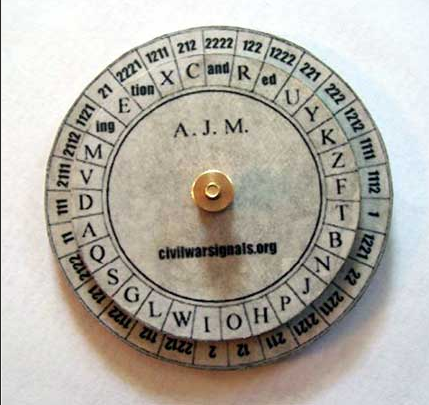
\includegraphics[width=0.6\textwidth]{img/cipher_disk.png}
\caption{Una de las muchas versiones del disco de cifrado. El alfabeto descrito en el círculo exterior puede cambiar para emplear diferentes símbolos si se desea. De la misma forma, el alfabeto descrito en el interior también puede cambiar añadiendo o eliminando grupos de palabras siendo que el alfabeto completo siempre debe estar presente. La posición de los discos en un momento dado nos dice qué símbolo del texto cifrado (círculo exterior) se corresponde con cada símbolo del texto original (círculo interior)}
\label{fig:cipher_disk}
\end{figure}

Como se observa en la figura \ref{fig:cipher_disk}, el disco de cifrado consta de dos círculos concéntricos. El círculo exterior está fijo mientras que el interior puede rotar, cambiando así su posición relativa respecto al exterior.

Hay dos formas de usar este instrumento. Podemos mantener los dos discos fijos a lo largo de todo el proceso de cifrado (resp. descifrado), con lo que estaríamos empleando un \textbf{criptosistema} de sustitución monoalfabética, o girar el disco interior periódicamente, con lo que estaríamos empleando un \textbf{criptosistema} de sustitución polialfabética.

Es necesario que el emisor y el receptor de la comunicación cifrada se pongan de acuerdo en la posición inicial de los discos y en la forma de girar los discos. Puede girarse el disco interior en sentido horario cada 10 caracteres, cada vez que venga una letra mayúscula, girarlo dos o tres posiciones en lugar de una y un largo etcétera de diversas combinaciones.

La idea original, desarrollada por \textbf{Alberti} era que la presencia de un número en el texto, introducido adrede, indicara el giro del disco interno. Este giro consistiría en colocar la letra que ha dado lugar al número debajo de la $A$ y continuar desde esa posición.

\subsubsection{Ataques contra cifrado de Alberti}

Los ataques contra este sistema se basan en el reconocimiento del caracter que representa un cambio de alfabeto de sustitución.

Una vez el atacante se hace con un texto cifrado y con el disco de cifrado correspondiente podrá reconocer de manera sencilla cuál es el caracter empleado.

\subsection{Criptosistema de Vigenere}
En el año 1518, \textbf{Johannes Trithemius} publicó el primer libro impreso acerca de la criptografía. En él se presenta el \textbf{cifrado de Trithemius} que acabaría dando lugar al \textbf{cifrado de Vigenere}.

El \textbf{cifrado de Trithemius} es un método de codificación polialfabético basado en el uso de la ``tabula recta'', un diagrama cuadrado de alfabetos donde cada fila se construye desplazando la anterior un espacio hacia la izquierda.

El siguiente ejemplo, extraído de Wikipedia, nos permite ilustrar el funcionamiento del \textbf{cifrado de Trithemius}.

La figura \ref{fig:tabula_recta} muestra cómo el mensaje original:
\begin{center}
``tabula recta''
\end{center}
se transforma en
\begin{center}
``TBDXOF XLKCK''
\end{center}
que resulta imposible de comprender si no se conoce el método de descifrado.

\begin{verbatim}
Texto original:  HISTORIA DE LAS MATEMÁTICAS
Clave: MATE
Texto cifrado:   SIMXARBE OE EEE MTXPMTXTCTW
\end{verbatim}

\begin{figure}[hbtp]
\centering
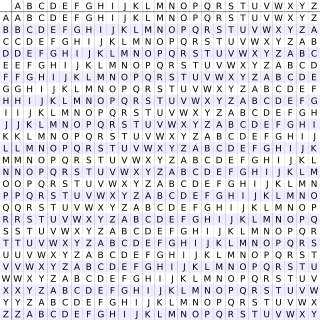
\includegraphics[width=0.6\textwidth]{img/tabula_recta.png}
\caption{Para codificar una palabra o mensaje se toma la primera letra y se codifica usando el \textbf{cifrado de César} asociado a la primera linea de la tabla. Tras esto pasamos a cifrar la segunda letra con el segundo \textbf{cifrado de César} de la tabla y así sucesivamente.}
\label{fig:tabula_recta}
\end{figure}

Este sistema tiene el \textbf{enorme inconveniente} de carecer de una clave secreta. Por tanto, tan pronto como alguien sepa que se está empleando este sistema, será perfectamente capaz de descifrar cualquier mensaje.

La idea de que no puede confiarse la seguridad del sistema en el desconocimiento de su funcionamiento así como la necesidad de basar los \textbf{criptosistemas} en una \textbf{clave} será formalizado por \textbf{Kerckkhoffs} en 1883 d.C. en lo que se conoce como el \textbf{principio de Kerkhoffs}:
\begin{center}
``Un criptosistema debe ser seguro cuando todo acerca del sistema es público excepto la clave.''
\end{center}

A fin de mejorar esta vulnerabilidad, en 1553 d.C. el italiano \textbf{Giovan Battista Bellaso} desarrolló una importante extensión del \textbf{cifrado de Trithemius} dando lugar al \textbf{cifrado de Vigenere}.

Este sistema se basa en la concatenación de diferentes \textbf{cifrados César} basándose en las letras de una palabra clave.

El uso de este \textbf{cifrado} parte de la definición de una palabra clave de longitud $n$ donde cada letra se interpreta como un número (de manera lógica siendo $A=0$) que será la clave de un \textbf{cifrado de César}. A partir del texto original y conociendo la \textbf{palabra clave} se cifra la primera letra con el \textbf{cifrado de César} correspondiente a la primera letra de la palabra clave y así sucesivamente. Al terminar de usar la última letra de la palabra clave, se vuelve a empezar.

\subsubsection{Ataque contra el criptosistema de Vigenere}
Para el atacante no es necesario conocer la palabra clave directamente sino que basta con conocer la longitud de esta. Una vez es sabido que se ha empleado una palabra de longitud $n$, basta con tomar aquellas letras situadas a distancia $n$ y analizarlas como resultado de un cifrado de César independiente que, recordemos, se realizaba por medio de un \textbf{análisis de frecuencias}.

La forma de atacar a este \textbf{criptosistema} no fue descubierta hasta el año 1920 d.C. cuando \textbf{William F. Friedman} desarrolló el concepto de \textbf{índice de coincidencia}.

El \textbf{índice de coincidencia} de un texto mide la probabilidad de que dos letras de un texto tomadas al azar coincidan. Por otro lado y de forma algo más abstracta, se define el \textbf{índice de coincidencia} de un idioma como la probabilidad de que dos letras, tomadas al azar de la totalidad de textos escritos en ese idioma, coincidan.

Si tomamos un texto cifrado y calculamos su índice de coincidencia con la fórmula:
\[I.C. = \sum_{i \in S}\mathbb{P}(i)\]
donde $S$ es el conjunto de letras diferentes presentes en el texto, obtendremos un valor similar al obtenido estudiando un texto compuesto por caracteres aleatorios. Es decir, suponiendo un alfabeto de 27 letras, al analizar el texto cifrado con el \textbf{cifrado de Alberti} obtendremos:
\[I.C. = 27 \times \left(\frac{1}{27}\right)^2 = \frac{1}{27} = 0.03\]

No obstante, si tomamos un texto correcto escrito en un idioma concreto, obtendremos un \textbf{índice de coincidencia} similar al del idioma en cuestión. Evidentemente, aunque se aplique un sistema de sustitución monoalfabética sobre el texto, el índice de coincidencia se mantiene intacto.

Así, si calculamos el \textbf{índice de coincidencia} del conjunto de letras cifradas con el mismo \textbf{cifrado de César}, es decir, aquellas a distancia $n$, obtendremos un valor similar al \textbf{índice de coincidencia} del texto original.

Una forma práctica de hacer esto consiste en tomar el texto cifrado y escribir debajo de él una copia del mismo. Una vez tenemos las letras dispuestas de esta forma desplazamos el texto inferior una posición a la derecha y comprobamos con que frecuencia letras colocadas una bajo la otra coinciden. Tras esto desplazamos una vez más y volvemos a calcular este valor y así sucesivamente.

Cuando se comparan letras a distancia $n$, siendo $n$ la longitud de la palabra clave, estamos considerando letras que han sido cifradas con el mismo \textbf{cifrado de César}.

Sean estas letras:
\[a_1a_2a_3,...,a_n\]
Cuando calculásemos el \textbf{índice de coincidencia} sobre esta secuencia de palabras estamos calculando:
\[I.C. = \frac{1}{(n-1)^2}\sum_{i=1}^n\sum_{j=1}^n\mathbb{1}_{\{a_i=a_j\}}\]

Por otro lado, el valor que se calcula al aplicar el procedimiento que acabamos de ver es:
\[α = \frac{1}{n-1} \sum_{i=1}^n \mathbb{1}_{\{a_i=a_{i+1}\}}\]

Puesto que el texto ha sido escogido al azar y estamos tomando simplemente una serie de caracteres del texto escogidos de forma aleatoria, es sencillo convencerse de que:
\[\forall j < n \ α \simeq \frac{1}{n-1}\sum_{i=1}^n\mathbb{1}_{\{a_i=a_{i+j}\}}\]

Teniendo esto en cuenta basta con escribir:
\[I.C. = \frac{1}{(n-1)^2}\sum_{i=1}^n\sum_{j=1}^n\mathbb{1}_{\{a_i=a_j\}} = \frac{1}{(n-1)^2}\sum_{i=1}^n \left( \mathbb{1}_{a_i=a_{i+1}} + ... + \mathbb{1}_{a_i=a_{i+n-1}}\right)\simeq\]
\[\simeq \frac{1}{(n-1)^2}\sum_{i=1}^n(n-1)\mathbb{1}_{a_i=a_{i+1}} = \frac{1}{n-1}\sum_{i=1}^n\mathbb{1}_{a_i=a_{i+1}}=α\]

Por tanto, llegados a cierto punto obtendremos un valor similar al \textbf{índice de frecuencia} del idioma en que fue escrito el texto y, sabiendo cuántos desplazamientos hemos realizado, conoceremos la longitud de la \textbf{palabra clave} empleada.

\subsection{La proliferación de la criptografía}
En Europa, la criptografía ganó, de forma secreta, importancia debido a la competencia entre las diferentes naciones y a la revolución religiosa. Durante el \textbf{Renacimiento}, los habitantes de diversos estados italianos  fueron responsables de la rápida proliferación de las técnicas de criptografía, algunas de las cuales reflejaban el entendimiento (o al menos el conocimiento) del \textbf{cifrado de Alberti}.

La criptografía, el criptoanálisis, los agentes secretos y la traición estuvieron presentes en el ``\textbf{Bablington plot}'': un complot para asesinar a la \textbf{Reina de Inglaterra, Elizabeth I} que acabó con la ejecución de \textbf{Mary, Reina de Escocia}.

Este complot tenía por objeto destituir a la \textbf{Reina Elizabeth}, una protestante, en favor de su prima \textbf{Mary}, reina de Escocia y católica. El objetivo a largo plazo era la invasión de Inglaterra por parte del \textbf{Rey Fernando II} de España.

El jefe de criptografía del \textbf{Rey de Francia Luis XIV} fue \textbf{Antonie Rossignol} y, junto con su familia, creó lo que hoy en día se conoce como el \textbf{Great Cipher} (en español, gran cifrado). Este nombre le fue asignado porque permaneció sin solución desde sus comienzos hasta la década de 1890 d.C. cuando el criptógrafo del ejército Francés \textbf{Etienne Bazeries} lo resolvió.

Fuera de Europa, cuando los Mongoles acabaron con la época de explendor de la cultura árabe, la criptografía se mantuvo, en comparación, estancada. En Japón no hay muestras del uso de la criptografía hasta 1510 d.C. y no emplearon técnicas avanzadas hasta la apertura del país hacia occidente a comienzos del año 1860 d.C.

\section{Desde 1800 hasta la Segunda Guerra Mundial}
Aunque la historia de la criptografía se remonta a tiempos de los romanos, no fue hasta el siglo XIX cuando comenzaron a desarrollarse técnicas complejas de cifrado y de criptoanálisis.

\subsection{Algunas personalidades de la época}
\subsubsection{Charles Babbage}
Un ejemplo de este desarrollo fueron los trabajos del matemático e ingeniero inglés \textbf{Charles Babbage} (December 1791 - October 1871), recordado por desarrollar el concepto de \textbf{ordenador programable}.

Considerado por algunos como \textbf{el padre de las computadoras}, \textbf{Babbage} inventó el primer computador mecánico que acabó dando lugar a diseños más complejos.

\textbf{Babbage} obtuvo notables resultados en criptografía que no fueron conocidos por el mundo hasta un siglo después de su muerte. Entre estos descubrimientos, a posteriori, se encontró que había resuelto un cifrado que había sido propuesto como un reto por su sobrino \textbf{Henry Hollier} y, en el proceso de desarrollo de esta solución, obtuvo importantes resultados relacionados con cifrados basados en las tablas de Vigenere. En concretó, observó que cifrar un texto con una \textbf{palabra clave} modificaba el texto de acuerdo a una aritmética modular.

Durante la \textbf{guerra de Crimea}, en 1850, \textbf{Babbage} consiguió romper el \textbf{cifrado de Vigenere} así como una versión mucho más compleja del mismo conocida como \textbf{cifrado de Vigenere de autoclave}, caracterizado por la incorporación del mensaje en la propia clave.

Este descubrimiento suponía un secreto militar por lo que no fue publicado. Unos años después, el oficial de infantería ruso \textbf{Friedrich Kasiski} logró el mismo resultado y lo publicó, con lo que obtuvo el crédito que debió corresponder a \textbf{Babbage}.

\subsubsection{Auguste Kerckhoffs}
En este época, el concepto de criptografía consistía en una serie de reglas consensuadas entre los expertos de la época.

Estas reglas permitían tener una idea ``objetiva'' de cuando un sistema de cifrado es bueno y cuando puede considerarse que ha sido superado.

El lingüista y criptógrafo \textbf{Auguste Kerkchoffs} (Enero 1835 - Agosto 1903) publicó una lista de seis principios que todo cifrado debía satisface:
\begin{enumerate}
\item El sistema debe ser, si no teóricamente irrompible, al menos irrompible en la práctica.
\item El diseño de un sistema no debe ser secreto y el conocimiento público del sistema no debe comprometer la seguridad del mismo. Es decir, la seguridad debe basarse en la secretitud de la clave, no del sistema o algoritmo de cifrado.
\item La clave debe poder ser memorizada y poder cambiarse con facilidad
\item Los criptogramas deben poder transmitirse por telégrafo
\item Los aparatos o documentos necesarios para llevar a cabo el proceso de cifrado o descifrado deber ser portátiles y operables por una única persona.
\item El sistema debe ser sencillo, sin requerir el conocimiento de una larga lista de reglas ni necesitar grandes ejercicios mentales.
\end{enumerate}

De entre estos seis principios el más conocido es el \textbf{segundo}, que ya mencionamos con anterioridad, conocido como \textbf{Principio de Kerckhoffs}

\subsubsection{Edgar Allan Poe}
El famoso escritor y crítico literario americano \textbf{Edgar Allan Poe} (Enero 1809 - Octubre 1849), conocido por su poesía y sus historias cortas centradas en lo misterioso y lo macabro, tuvo también una importante contribución a la criptografía.

Los intereses en \textbf{criptografía} de este escritor así como su habilidad en el campo, quedaron constatados en un artículo publicado en el periódico de Philadelfia ``Alexander's Weekly (Express) Messenger'' en el que invitaba a que le enviasen cifrados que el procedería a resolver.

Fomentó enormemente el interés público por la \textbf{criptografía} con su obra ``The Gold-Bug'', un pequeño relato que incorporaba cifrados como parte esencial de la historia.

La importantísima aportación de este escritor a la \textbf{criptografía} no se basa en un profundo conocimiento de la misma sino en su conocimiento de la cultura periodística. Fue consciente de lo ignorante que era el público general acerca de la criptografía y trató de fomentar su interés por la misma.

Sus historias incentivaron a muchas personas a entrar en el mundo de la criptografía. Un ejemplo de esta influencia es \textbf{William Friedman}, uno de los más famosos criptólogos de todo América quien confirmó en diversas ocasiones que fue la obra ``The Gold-Bug'' la que incentivó su interés por la \textbf{criptografía}.

\subsection{Primera Guerra Mundial}
Durante la Primera Guerra Mundial, la \textbf{habitación 40}, también conocida como 40 O.B. (Old Building) era la sección del almirantazgo británico que lideró los esfuerzos de Inglaterra en el campo del criptoanálisis durante la Primera Guerra Mundial.

Fue la \textbf{habitación 40} quien rompió los códigos navales empleados por los alemanes, jugando así un rol importantísimo en los enfrentamientos navales de esta guerra. Así, por ejemplo, se descubrió la salida de la flota alemana al mar del Norte donde los ingleses enviaron sus tropas para interceptarla dando lugar a las batallas de \textbf{Dogger Bank} y \textbf{Jutland}.

No obstante, la mayor aportación en el ámbito de la criptografía fue descifrar el \textbf{Zimmermann Telegram}, un mensaje enviado desde la Oficina de Asuntos Exteriores de Alemania, via Washington, al embajador \textbf{Heinrich von Eckardt} en México, lo que tuvo un gran peso en la decisión de Estados Unidos de entrar en la guerra.

\subsubsection{Cifrado de transposición}
El sistema de cifrado empleado en el \textbf{Zimmermann Telegram} era una versión del \textbf{cifrado de transposición} mucho más compleja.

En un \textbf{cifrado de transposición} las letras del texto en claro son reordenadas de acuerdo a una cierta regla acordada previamente. Una técnica habitual consiste en dividir el texto en bloques de una longitud dada y reordenar las letras de cada bloque siguiendo una regla definida por una palabra clave.

El proceso consiste en tomar la palabra clave, eliminar las letras repetidas, con lo que obtendremos una palabra de tamaño $n$, y ordenar estas letras alfabéticamente. Una vez se ha hecho esto, se divide el texto en claro en bloques de tamaño $n$ y se reordena cada bloque del texto como se reordenó la clave.

Por último, para dificultar los ataques, se envía en texto cifrado dividido en bloques de longitud distinta a $n$.

Así, el texto:
\begin{center}
ESTE TRABAJO ES MUY BUENO
\end{center}
tomando la palabra clave ``FACULTAD'' se cifrará dividiéndolo en bloques de tamaño $n=7$ puesto que las letras diferentes de la clave forman: ``FACULTD''.

El mensaje original dividido de manera adecuada queda
\begin{center}
ESTETRA BAJOESM UYBUENO
\end{center}

La reordenación a aplicar en cada bloque es la correspondiente a:
\begin{center}
FACULTD -> ACDFLTU
\end{center}

Tras aplicar esta reordenación el mensaje queda:
\begin{center}
STAETRE AJMBESO YBOUENU
\end{center}

Finalmente, escribiendo el texto de manera que no de pistas sobre el valor $n$ utilizado se obtiene el mensaje cifrado:

\begin{center}
STAET REAJM BESOY BOUEN U
\end{center}

\subsubsection{Ataque contra el cifrado de transposición}
Es sencillo de detectar cuando se está empleando un \textbf{cifrado de transposición} puesto que cambiar el orden de las letras no cambiar la frecuencia de ocurrencia de las mismas. Así, una \textbf{característica clave} de un \textbf{cifrado de transposición} es que cada letra aparece con la frecuencia asociada a dicha letra en el idioma en que fue escrito.

A fin de poder descifrar un mensaje interceptado con este cifrado, hay que deducir el tamaño de los bloques y la reordenación adecuada.

Aquí encontramos la primera debilidad del \textbf{cifrado de transposición}: Los bloques usados para dividir el texto original deben tener un tamaño $n$ que divida al tamaño del mensaje original.

En caso de que se haya completado el texto con caracteres extra para alcanzar una longitud múltiplo de $n$, se observarían en la parte final del código una densidad mayor de la debida de un cierto tipo de caracter.

Una vez se estima cuál puede ser el valor de $n$ utilizado, hay que experimentar con diferentes reordenaciones posibles.

La \textbf{principal debilidad} de este sistema es que las letras empleadas en el mensaje original están todas en el mensaje cifrado, lo que facilita las técnicas de criptoanálisis.

Una opción es tratar de formar una primera palabra con sentido con las letras iniciales del mensaje cifrado y aplicar la misma reordenación al resto del mensaje.

Otra posibilidad, es conocer una palabra que aparezca seguro en el mensaje. Cuanto mayor sea la longitud de la palabra mejor será. Una vez se conoce que una determinada palabra está en el mensaje original, basta con buscar las letras de la palabra en el mensaje lo que nos da una idea de la ordenación empleada y del valor $n$.

Vamos a ilustrar estas ideas con un ejemplo que ``imita'' el \textbf{Zimmermann telegram}, extraido de \cite{Wikipedia:ZimmermanExample}.

El mensaje cifrado que fue interceptado por los ingleses decía:
\begin{center}
\begin{tabular}{ccccccc}
HIIFA & STMPT & TITET & SSNCU & OSFCE & LUSRO & WEOPP\\
NASEL & LACEI & ANONF & OTHLL & ENGOW & ABIWI & SIHTS\\
ICMET & OXWEH & AHSTM & AALEK & LTOWA & EGRRA & THDNE\\
ETTOE & HGKER & MEPAW & EACHS & EGIAL & EVLER & GELAN\\
ANFII & CNUPA & LOPSN & DRTTI & ANDIS & REUOD & STHTO\\
EXATC & IMTOO & IERSQ & UCORE & NLOTH & TSERI & TEOTR\\
NNRYW & EIICM & ETOXS & AEXDN & AZOAR & ANIDE & THATE\\
ARILL & ESTOE & FOYTR & SUFTE & OMETL & TNE &
\end{tabular}
\end{center}

El texto se compone de 273 letras. Puesto que
\[273 = 3 \times 7 \times 13\]
los únicos factores posibles son $1$, $3$, $7$, $13$, $21$, $39$, $91$ y $273$.

De estos factores, el más probable es el número $7$ pues debe relacionarse con el número de letras diferentes de una palabra sencilla de memorizar. $1$ y $3$ son valores demasiado pequeños puesto que dejan el texto fácilmente reconocible y a partir de $13$ empieza a ser demasiado grande.

Reorganizando el mensaje en bloques de tamaño $7$ este queda:
\begin{center}
\begin{tabular}{ccccc}
HIIFAST & MPTTITE & TSSNCUO & SFCELUS & ROWEOPP\\
NASELLA & CEIANON & FOTHLLE & NGOWABI & WISIHTS\\
ICMETOX & WEHAHST & MAALEKL & TOWAEGR & RATHDNE\\
ETTOEHG & KERMEPA & WEACHSE & GIALEVL & ERGELAN\\
ANFIICN & UPALOPS & NDRTTIA & NDISREU & ODSTHTO\\
EXATCIM & TOOIERS & QUCOREN & LOTHTSE & RITEOTR\\
NNRYWEI & ICMETOX & SAEXDNA & ZOARANI & DETHATE\\
ARILLES & TOEFOYT & RSUFTEO & METLTNE &
\end{tabular}
\end{center}

Puesto que el mensaje ha sido enviado a México, parece razonable asumir que la palabra MEXICO aparecerá en el texto. Así, puede verse que hay tres bloques distintos donde aparecen todas o casi todas las letras que componen la palabra MEXICO:

\begin{center}
\begin{tabular}{ccccc}
HIIFAST & MPTTITE & TSSNCUO & SFCELUS & ROWEOPP\\
NASELLA & CEIANON & FOTHLLE & NGOWABI & WISIHTS\\
\textbf{ICMETOX} & WEHAHST & MAALEKL & TOWAEGR & RATHDNE\\
ETTOEHG & KERMEPA & WEACHSE & GIALEVL & ERGELAN\\
ANFIICN & UPALOPS & NDRTTIA & NDISREU & ODSTHTO\\
\textbf{EXATCIM} & TOOIERS & QUCOREN & LOTHTSE & RITEOTR\\
NNRYWEI & \textbf{ICMETOX} & SAEXDNA & ZOARANI & DETHATE\\
ARILLES & TOEFOYT & RSUFTEO & METLTNE &
\end{tabular}
\end{center}

Por último, sabiendo que el mensaje está escrito en inglés, parece razonable asumir que el bloque ``EXATCIM'' en realidad es ``ATMEXICO''. Extendiendo esta asunción pueden reordenarse todos los bloques obteniendo el mensaje:

\begin{center}
``If this attempt is not successful we propose an alliance on the following basis with Mexico: that we shall make war together and together make peace. We shall give general financial support and it is understood that Mexico is to reconquer the lost territory in New Mexico, Texas, and Arizona. The details are left to you for settlement.''
\end{center}

\subsubsection{Zimmermann Telegram}
Sobre las diez y media de la mañana del 17 de Enero de 1917, \textbf{William Montgomery}, un estudiante que estaba sirviendo al cuerpo de criptoanalistas de la \textbf{Habitación 40} encontró lo que parecía ser un importante mensaje.

Sus instintos eran ciertos, el criptograma que encontró el joven, y que leyó parcialmente junto a su compañero \textbf{Nigel de Grey}, se convertiría en el \textbf{cifrado} con la solución más difícil de alcanzar y más importante de la historia.

Se trataba de un mensaje largo, compuesto por unos mil bloques de números. Datado del 16 de Enero en Berlín, estaba dirigido al embajador alemán de los Estados Unidos, \textbf{Count Johann Heinrich Andreas Von Bern-storff} y los dos criptoanalistas se percataron de que estaba cifrado con un código diplomático alemán conocido como 0075, cifrado sobre el que llevaban seis meses trabajando.

Los criptógrafos de la \textbf{Habitación 40} sabían, por sus previos análisis, que el \textbf{cifrado 0075} pertenecía a una serie de cifrados de dos partes que la Oficina de Asuntos Exteriores alemana designaba con dos ceros y dos dígitos, donde los dos dígitos siempre siempre tenían diferencia igual a 2.

Entre otros, algunos de los cifrados de esta familia que ya habían resuelto eran 0097, 0086, 0064, etc. El \textbf{cifrado 0075} era un código nuevo que la Oficina de Asuntos Exteriores alemana había distribuido por primera vez en Julio de 1916 para las misiones alemanas en Viena, Sofía, Constantinopla, Bucarest, Copenague, Estocolmo, Berna y Oslo. De algún modo los británicos lograron hacerse con suficientes mensajes cifrados con este sistema para conseguir que \textbf{Montgomery} y \textbf{de Grey} lograran romper el cifrado.

Tal y como se describe en \cite{Book:TelegraphDiplomacy}, el \textbf{código 0075} consiste en unas 10,000 palabras o frases, ordenadas de forma aleatoria, cada una de las cuales se corresponde con un número entre 0000 y 9999.

Romper un código así desde cero requiere identificar los bloques que representan las palabras más comunes. Aunque estos códigos trataban de defenderse de este tipo de ataques definiendo múltiples bloques para representar las palabras mas comunes, quienes escribían los mensajes tendían a aprender uno o dos bloques para esas palabras y a usarlos repetidamente.

Una de los primeros bloques que se consiguió identificar, debido a la frecuencia de sus apariciones, era el que representaba la palabra ``STOP''. Una vez fueron capaces de detectar las apariciones de esta palabra en los telegramas cifrados que interceptaban, pudieron reconocer los límites de las frases para aplicar sobre ellos análisis sintácticos.

También pudieron identificar frases y expresiones comunes utilizadas por los embajadores comenzando así a descifrar el mensaje poco a poco.

Evidentemente toda esta tarea fue posible debido a que disponían de una gran cantidad de mensajes cifrados con lo que las estadísticas podían funcionar.

\section{Segunda Guerra Mundial}
Durante el desarrollo de la Segunda Guerra Mundial, se disparó el uso de máquinas de cifrado mecánicas y electromagnéticas aunque se siguieron utilizando los sistemas manuales en las ocasiones en que estas máquinas no podían usarse.

A lo largo del conflicto se produjeron importantes avances en el campo del diseño de cifrados y el criptoanálisis aunque, de forma evidente, estos avances se mantuvieron en secreto y no fueron mostrados al público hasta 50 años después.

Los alemanes hicieron uso de una máquina de cifrado llamada \textbf{Enigma}, cuyos detalles veremos a continuación. El matemático polaco \textbf{Marian Rejewski} logró, en diciembre de 1932, deducir la estructura detallada de la máquina \textbf{Enigma} apoyándose en las matemáticas y en la limitada documentación proporcionada por el capitán \textbf{Gustave Bertrand} del servicio de inteligencia francés.

\subsection{Enigma}
La máquina \textbf{Enigma} fue inventada y desarrollada por el ingeniero alemán \textbf{Arthur Scherbius} hacia el final de la Primera Guerra Mundial. Los primeros modelos salieron al mercado a principios de 1920 y fueron adoptados por el gobierno y el ejército alemán. Esta máquina fue explotada, fundamentalmente, por la Alemania Nazi antes y durante el desarrollo de la Segunda Guerra Mundial.

Mensajes militares alemanes cifrados con \textbf{Enigma} fueron descifrados por primera vez por el \textbf{Cipher Bureau} polaco: agencia de Polonia centrada en el estudio de la criptografía. Este logro se debe a los esfuerzos de tres matemáticos polacos: \textbf{Marian Rejewski}, \textbf{Jerzy Rozycki} y \textbf{Hernyk Zygalsky} quienes, apoyándose en principios matemáticos, lograron deducir el funcionamiento de la máquina a partir de los mensajes cifrados.

A partir de 1938, los alemanes fueron añadiendo complejidad a la máquina haciendo que el trabajo de los polacos quedará anticuado.

\subsubsection{Principios básicos}

Aunque se desarrollaron muchos modelos de \textbf{Enigma}, que añadían complejidad, de forma incremental, al modelo original, vamos a centrarnos en la estructura de uno de los últimos modelos por ser este el más completo y famoso de todos.

La máquina \textbf{Enigma} producía un \textbf{cifrado polialfabético de sustitución}. Durante la Primera Guerra Mundial, de manera simultánea en diferentes países, los inventores y matemáticos se dieron cuenta de que una clave completamente aleatoria que no contuviera ningún patrón repetitivo, en principio, haría este tipo de cifrado irrompible.

Esto llevó al desarrollo de máquinas de cifrado con rotores que tras pulsar una letra del texto original, producían una letra cifrada, cambiando los caminos que seguía la señal eléctrica por medio de los rotores. Además, tras cada letra pulsada la posición de los rotores cambiaría haciendo que la siguiente letra fuera cifrada con un cifrado diferente.

\subsubsection{Estructura de Enigma}

La figura \ref{fig:enigma} muestra el esquema de funcionamiento de la máquina \textbf{Enigma}, donde el número 8 representa uno de los modificadores, que simplemente conectaba pares de letras para que fuesen intercambiadas; el número 5 representa los rotores y el número 6 el reflector.

\vspace{1cm}

\begin{minipage}{0.5\textwidth}
\begin{center}
%\centering
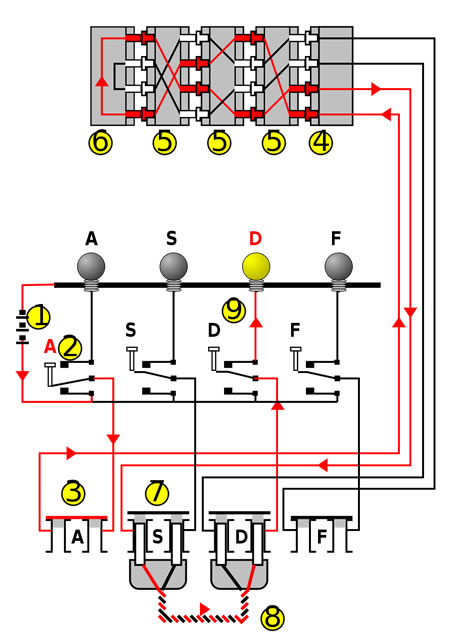
\includegraphics[width=\textwidth]{img/enigma.jpg}
\captionof{figure}{Estructura de Enigma}
\label{fig:enigma}
\end{center}
\end{minipage}
\begin{minipage}{0.45\textwidth}
Tras finalizar el cifrado de la letra $A$, los rotores girarían de modo que no se volvería a seguir el mismo camino nunca más. Los componentes principales de la estructura son:
\begin{enumerate}
\item Batería.
\item Conexión con el teclado.
\item Conexión de modificador.
\item Rueda de entrada.
\item Rotores.
\item Reflector.
\item Conexión de modificador.
\item Modificador.
\item Bombilla que representa la letra cifrada.
\end{enumerate}
\end{minipage}

\vspace{1cm}

En rojo se muestra el flujo que seguiría la corriente en caso de pulsar la letra $A$, que, según este ejemplo, sería cifrada a una $D$.

Para poder emplear la máquina era necesario conocer:
\begin{itemize}
\item \textbf{La estructura interna de la máquina}, que está fijada una vez sabemos qué máquina se está empleando.
\begin{itemize}
\item Las conexiones entre el teclado y la entrada de corriente a la máquina.
\item Las conexiones de cada rotor.
\item El número y la posición de las muescas en los anillos de cada rotor.
\item Las conexiones de los reflectores.
\end{itemize}

\item \textbf{Configuración interna}, que puede cambiar aunque con poca frecuencia lo hace.
\begin{itemize}
\item Los rotores utilizados y la posición relativa de los mismos.
\item La disposición de las letras del teclado.
\end{itemize}
\item \textbf{Configuración externa}, que pueda cambiar y lo hace con frecuencia.
\begin{itemize}
\item La posición de los modificadores
\item La posición de los rotores al comienzo de la transmisión del mensaje.
\end{itemize}
\end{itemize}


\subsubsection{Seguridad de la máquina}
Los diferentes modelos desarrollados de esta máquina tenían diferentes niveles de seguridad. La clave de la seguridad de estas máquinas era la enorme cantidad de combinaciones posibles de cifrado de cada letra, lo que hacía imposibles los ataques por fuerza bruta.

Además de las capacidades de la máquina en sí misma, tenía otra ventaja. Había ciertas componentes que se modificaban manualmente a la hora de usar la máquina, es decir, la máquina podía configurarse.

Por ejemplo, era posible modificar la posición inicial de los rotores e incluso cambiar unos rotores por otros. Por otro lado, las conexiones que permitían el intercambio de dos letras podían colocarse entre cualquier par de letras.

Analizando la máquina de la figura \ref{fig:enigma} y considerando un alfabeto compuesto por 26 letras, con 5 rotores de entre los que hay que escoger 3 y modificando 6 pares de letras\footnote{Es decir, tenemos 6 modificadores}, la pregunta que surge es clara, ¿Cuántos cifrados distintos pueden obtenerse?, es decir, a partir de un mismo texto en claro, ¿Cuántos cifrados distintos pueden obtenerse según la configuración de la máquina?.

En primer lugar hay que escoger qué tres rotores de entre los 5 disponibles. Teniendo en cuenta que importa el orden, tenemos un total de:
\[5 \times 4 \times 3 = 60 \text{ posibilidades}\]

Una vez se han escogido los rotores, debemos ver qué posición tendrá cada rotor. Puesto que hay 26 posiciones para cada rotor tenemos un total de
\[26\times 26 \times 26 = 26^3 \text{ posibilidades}\]

Por último deben colocarse los modificadores, para lo que hay que elegir 6 pares de letras. Esto nos lleva a tener un total de
\[\frac{1}{6!}{26 \choose 2} \cdot {24\choose 2}\cdot {22\choose 2}\cdot {20\choose 2}\cdot {18\choose 2}\cdot {16\choose 2} \text{ posibilidades }\]

donde la primera fracción se deriva del hecho de que no importa el orden en que los coloquemos.

Combinando estas operaciones obtenemos que la máquina \textbf{Enigma} consta de un total de
\[\frac{60\cdot 26^3 \cdot {26 \choose 2} \cdot {24\choose 2}\cdot {22\choose 2}\cdot {20\choose 2}\cdot {18\choose 2}\cdot {16\choose 2}}{6!}\approx 8.469 \cdot 10^{17}  \text{ claves diferentes}\]

\subsection{Debilidad de Enigma}

Si toda la flota empleaba el mismo sistema de cifrado y los mensajes eran fácilmente interceptables (puesto que se comunicaban por radio) al final sería relativamente sencillo que el enemigo descifrara la clave si utilizaban siempre la misma.
%
Para solucionar esto, lo que se hacía era modificar diariamente la clave utilizada y disponer de un libro de claves en el que se establecía qué configuración de la máquina correspondía a qué día.
%
Además, este libro era diferente para cada mes, de tal manera que si el enemigo se hacía con un libro, sólo podría descifrar los mensajes de lo que quedara de mes.


Ante un sistema así, ¿cómo se puede romper?
%
El gran problema que puso en peligro la seguridad del sistema era el hecho de que el primer mensaje del día siempre informaba del tiempo atmosférico, lo que supone una información muy valiosa para el atacante, que vería facilitadas sus labores de criptoanálisis.
%
Todos los comienzos de mensajes incluirían la palabras "tiempo", "presión atmosférica", "informe"... 
%
La labor de descifrar se reduce notablemente, aunque seguía siendo una tarea muy difícil.


\subsubsection{Descifrado de mensajes con Enigma}
A la hora de descifrar un mensaje, el mecanismo es sencillo puesto que el funcionamiento de \textbf{Enigma} está basada en transposiciones. Es decir, si a partir de la letra $A$ se obtiene la $B$, a partir de la $B$ se obtendrá la $A$, partiendo de la misma clave.

Por tanto, una vez recibido el mensaje lo único que hay que hacer es introducir el mensaje cifrado en la máquina y como salida se obtiene el texto original.

Para comprobar que la función de cifrado y su inversa son la misma, basta con analizar cómo funcionaba \textbf{Enigma} sobre cada letra.

En primer lugar se intercambiaba una letra por otra mediante los modificadores. Tras esto la letra pasa por los rotores y llega al reflector (que será la clave de la demostración) y tras ello vuelve a pasar por los rotores y por el modificador.

Así se obtiene:
\[\rho(m) = σ^{-1}δ^{1}Rδσ(m) \implies \rho^{-1}(m) = σ^{-1}δ^{1}Rδσ(m) = \rho(m)\]

Esto da lugar a otra ``debilidad'' del cifrado con \textbf{Enigma} y es que la cantidad de claves que hemos calculado anteriormente no se corresponde con la situación real.

De todas las claves posibles que mencionamos al inicio de esta sección, no todas darán lugar a una función $\rho$ que coincida con su inversa.

Sabiendo que la máquina funciona por transposiciones, podemos escribir:
\[\rho = \rho^{-1} \iff \rho = (a_1a_2)(a_3a_4)...(a_{25}a_{26})\]
puesto que necesitamos que $\rho$ no haga más que permutar pares de letras.

Dada esta restricción podemos calcular un total de
\[\frac{{26 \choose 2} \cdot {24 \choose 2} \cdot ... \cdot {2 \choose 2}}{13!} =\frac{26!}{13!2^{13}} \approx 1.01 \cdot 10^{15} \text{ claves posibles }\]
que sigue siendo un número muy elevado pero es notablemente inferior al calculado sin considerar esta restricción.

Otra importante \textbf{debilidad} del sistema es que una letra \textbf{nunca sería cifrada a sí misma}. Esta propiedad resultaba muy útil a la hora de buscar en el mensaje cifrado pequeños fragmentos de texto que se espera se hayan usado en el texto original, puesto que permitía eliminar regiones del texto cifrado.

Si se considera que una cierta porción del mensaje cifrado se corresponde con un cierto texto original y una sola letra queda inmutada, puede descartarse. Esta idea fue explotada por el matemático \textbf{Alan Turing} en el desarrollo de la \textbf{Bomba Británica}, la máquina que logró derrotar a \textbf{Enigma}.

Por otro lado, los modificadores eran recíprocos. Si la letra $A$ se intercambiaba con la $B$, la $B$ se intercambia con la $A$. Esta propiedad indujo al matemático \textbf{Gordon Welchman} a introducir un tablero diagonal en \textbf{La Bomba}, reduciendo enormemente el número de pruebas erróneas que hacía esta.

En definitiva, aunque el cifrado sufría de algunas debilidades, la clave de la victoria en la lucha por descifrarlo se basa en fallos humanos en el uso práctico del sistema.

Al final de la guerra, el 19 de abril de 1945, los altos mandos del ejército británico recibieron orden de no revelar al mundo que el \textbf{cifrado Enigma} había sido resuelto, pues esto daría pie al derrotado enemigo a clamar que ``la derrota no habría sido justa''.

\subsection{Otros cifrados importantes en la Segunda Guerra Mundial}
Los alemanes también lograron algunos éxitos en el campo del criptoanálisis resolviendo, por ejemplo, el \textbf{Cifrado Naval Nº 3}. Esto permitió a los alemanes atacar y hundir convois Atlánticos.

Esté código estuvo resuelto por los alemanes hasta el cuarto año de guerra, momento en que los ingleses decidieron cambiar el sistema. Sin embargo, la organización descentralizada del ejército alemán dio lugar a una enorme duplicación de esfuerzos, pues se disponía de numerosas unidades dedicadas a la criptografía que trabajaban de forma aislada.

También fueron de vital importancia los códigos empleados por los Japoneses, entre los que destaca el $JN-25$. Este código fue resuelto por la armada americana tras una ardua tarea de criptoanálisis.

Este cifrado se componía de dos libros. El primero de ellos contenía el código en si mismo; el segundo, una serie de cifrados extra que eran aplicados a los códigos antes de transmitirlos.

En el bando aliado podemos encontrar la máquina \textbf{TypeX} británica y la americana \textbf{SIGABA}. Ambas eran máquinas electromecánicas que funcionaban por medio de rotores de forma similar a la máquina \textbf{Enigma}.

Por último cabe destacar el sistema empleado por la Unión Soviética: el \textbf{cifrado VIC}. El sistema consistía en la selección de un texto aleatorio de igual longitud que el texto que se desea enviar.

Una vez tenemos el texto original y el texto aleatorio, se escriben ambos en binario y combinan bit a bit por medio de una suma binaria en cada bit, es decir, una puerta lógica XOR.

Si el texto aleatorio era realmente un texto aleatorio, sin ningún patrón claro, el resultado de esta operación sería una secuencia de bits aleatorios.

Este sistema de cifrado se considera un \textbf{cifrado perfecto} siempre y cuando el texto aleatorio no se reutilice, ni se reutilicen partes del mismo. No obstante, este sistema presenta el gran inconveniente de la necesidad de compartir una enorme cantidad de claves a fin de poder mantener una comunicación.

\section{Edad Contemporánea}
La criptografía en los tiempos contemporáneos se basa en el uso de algoritmos que emplean una clave para cifrar y descifrar información. 
%
En general, cuanto más larga es esta clave más difícil es romper el algoritmo.

Este aumento de dificultad junto al tamaño de la clave se debe a que los ataques por fuerza bruta requieren probar todas las posibles claves, actividad que se vuelve notablemente más costosa cuanto mayor es la clave, pues mayor será el número de posibilidades.

Desde la Segunda Guerra Mundial, el mayor avance en el campo de la criptografía es el desarrollo de los \textbf{criptosistemas de clave pública}.

A comienzos de los 90, el uso de internet con fines comerciales y la introducción del comercio electrónico supuso una llamada al desarrollo de nuevos sistemas de cifrado. Así surgió el \textbf{Data Encryption Standard (DES)}, un sistema de \textbf{clave simétrica}.

\subsection{Claude Shannon}
\textbf{Claude E. Shannon} es considerado el \textbf{padre de la criptografía matemática}. Shannon trabajó durante años en los laboratorios Bell donde publicó, en 1949, un artículo de título: ``A mathematical theory of cryptography''. Shannon continuó este trabajo publicando el artículo: ``A mathematical theory of communication'', considerado como el \textbf{punto de partida de la criptografía moderna}.

En sus trabajos \textbf{Shannon} describe los dos tipos básicos de sistemas de seguridad:
\begin{itemize}
\item Sistemas desarrollados con el objetivo de protegerse contra atacantes que disponen de absolutamente todos los recursos necesarios para descifrar un mensaje. Es decir, se trata de sistemas que deben ser seguros desde el punto de vista teórico.
\item Sistemas desarrollados con el objetivo de protegerse contra atacantes que disponen de una cantidad limitada de recursos para descifrar un mensaje. Nos encontramos ante sistemas que deben ser seguros desde el punto de vista práctico.
\end{itemize}

\textbf{Shannon} centró su trabajo en el estudio del primer tipo de sistemas y desarrolló el concepto de \textbf{irrompibilidad de un cifrado}. Si un cifrado se considera \textbf{irrompible} se considera que es \textbf{perfecto}. \textbf{Shannon} concluyó que la seguridad perfecta sólo podía obtenerse empleando claves \textbf{secretas y de un único uso} cuya longitud fuese mayor o igual que el mensaje a transmitir

\subsection{DES: Data Encryption Standard}
Los sistemas de cifrado de clave simétrica se caracterizan por el uso de una misma clave tanto para cifrar como para descifrar mensajes.

Todos los criptosistemas vistos hasta este momento a lo largo de este documento son cifrados de clave simétrica: una vez se tiene la información necesaria para cifrar un mensaje, se tiene la información necesaria para descifrarlo.

Con la llegada de internet y la extensión de su uso más allá de las universidades, surgió la preocupación por la seguridad informática. Así se desarrolló el estándar DES que fue aceptado por la \textbf{National Security Agency} el 15 de julio de 1977.

El DES era un sistema de cifrado por bloques, es decir, operaba sobre bloques de texto plano de 64 bits. Así, el resultado de este cifrado es una \textbf{permutación} de los bits en bloques de longitud 64.

El algoritmo parte de bloques de 64 bits del texto original, que parte por la mitad formando un bloque izquierdo, que denotamos \textbf{L} y uno derecho, \textbf{R}, cada uno de los cuales compuesto por 32 bits.

Una vez hecho esto, los pasos que sigue el algoritmo son:
\begin{enumerate}
\item \textbf{Creación de 16 subclaves, cada una de 48 bits}.

Para ello empezamos tomando sólo 56 bits de la clave de acuerdo con la siguiente tabla.

\begin{center}
\begin{tabular}{ccccccc}
57 &  49 &   41 &  33 &   25  &  17 &   9\\
1  & 58  &  50  & 42  &  34   & 26  & 18\\
10 &   2 &   59 &  51 &   43  &  35 &  27\\
19 &  11 &    3 &  60 &   52  &  44 &  36\\
63 &  55 &   47 &  39 &   31  &  23 &  15\\
7  & 62  &  54  & 46  &  38   & 30  & 22\\
14 &   6 &   61 &  53 &   45  &  37 &  29\\
21 &  13 &    5 &  28 &   20  &  12 &   4
\end{tabular}
\end{center}

Es decir, formamos una nueva clave tomando los bits 57, 49, etc de la clave original.

Tras esto dividimos la clave en dos mitades: la izquierda que denominamos $C_0$ y la derecha, $D_0$.

Una vez se definen $C_0$ y $D_0$ procedemos a definir 16 pares de cadenas $C_n$ y $D_n$ con $n = 1, ..., 16$ donde cada par se obtiene a partir del anterior realizando un desplazamientos según indica la siguiente tabla

\begin{center}
\begin{tabular}{cc}
Iteración & Desplazamientos a la izquierda \\
\hline
1  & 1 \\
2  & 1 \\
3  & 2 \\
4  & 2 \\
5  & 2 \\
6  & 2 \\
7  & 2 \\
8  & 2 \\
9  & 1 \\
10 &  2 \\
11 &  2 \\
12 &  2 \\
13 &  2 \\
14 &  2 \\
15 &  2 \\
16 &  1
\end{tabular}
\end{center}

Uniendo de nuevo las cadenas $C_n$ con su respectiva $D_n$ se obtiene 16 claves, $K_n$, de de 58 bits, de las que se seleccionan 48 bits concretos según la siguiente tabla:

\begin{center}
\begin{tabular}{ccccccc}
14 &  17 &  11 & 24 &   1 &   5 \\
3  & 28  & 15  & 6  & 21  & 10 \\
23 &  19 &  12 &  4 &  26 &   8 \\
16 &   7 &  27 & 20 &  13 &   2 \\
41 &  52 &  31 & 37 &  47 &  55 \\
30 &  40 &  51 & 45 &  33 &  48 \\
44 &  49 &  39 & 56 &  34 &  53 \\
46 &  42 &  50 & 36 &  29 &  32
\end{tabular}
\end{center}

\item \textbf{Ciframos cada bloque de 64 bits}.

Para empezar se permutan los 64 bits del bloque de texto claro de acuerdo a la siguiente tabla:

\begin{center}
\begin{tabular}{cccccccc}
58 & 50 & 42 & 34 & 26 & 18 & 10 & 2\\
60 & 52 & 44 & 36 & 28 & 20 & 12 & 4\\
62 & 54 & 46 & 38 & 30 & 22 & 14 & 6\\
64 & 56 & 48 & 40 & 32 & 24 & 16 & 8\\
57 & 49 & 41 & 33 & 25 & 17 &  9 & 1\\
59 & 51 & 43 & 35 & 27 & 19 & 11 & 3\\
61 & 53 & 45 & 37 & 29 & 21 & 13 & 5\\
63 & 55 & 47 & 39 & 31 & 23 & 15 & 7
\end{tabular}
\end{center}

y dividimos el bloque resultante en dos mitades, que denotamos como $L_0$ y $R_0$ (mitad izquierda y derecha respectivamente).

Tras esto se procede a realizar 16 operaciones según la ecuación:
\[\begin{array}{l}
L_n = R_{n-1} \\
R_n = L_{n-1}+f(R_{n-1},K_n)
\end{array}\]

donde la función $f(x,y)$ se define como:
\[f(x,y) = \text{SBOX}(E(x) \text{XOR} y)\]
donde $E(x)$ representa una expansión de la cadena $x$ hasta alcanzar 48 bits. Esta expansión se lleva a cabo utilizando la siguiente tabla:
\begin{center}
\begin{tabular}{ccccccc}
32 &  1 &   2 &   3 &   4 &   5\\
4  & 5  &  6  &  7  &  8  &  9\\
8  & 9  & 10  & 11  & 12  & 13\\
12 & 13 &  14 &  15 &  16 &  17\\
16 & 17 &  18 &  19 &  20 &  21\\
20 & 21 &  22 &  23 &  24 &  25\\
24 & 25 &  26 &  27 &  28 &  29\\
28 & 29 &  30 &  31 &  32 &   1
\end{tabular}
\end{center}

La función SBOX toma bloques de 6 bits de la cadena de 48 bits que recibe como argumento y los convierte en cadenas de 4 bits. Esta operación se realiza mediante el uso de tablas, una distinta para cada bloque de 6 bits.


\end{enumerate}

El proceso de descifrado se realiza siguiendo los mismo pasos en orden inverso.

Finalmente, con el avance de los ordenadores, este sistema acabó siendo vulnerable a ataques de fuerza bruta, problema que se resuelve empleando una clave más larga.

\subsection{Criptosistema de clave asimétrica}
Cuando el internet comenzó a desarrollarse al punto de que todo el mundo tenía acceso, comenzaron a desarrollarse cientos de aplicaciones que requerían el establecimiento de comunicaciones seguras.

El primer problema con las claves simétricas fue la imposibilidad de establecer una clave para cada par de personas que quieren comunicarse de manera segura así como la dificultad de la compartición de esta clave.

Por otro lado, el sistema \textbf{DES} era vulnerable si se empleaban claves pequeñas, pero las personas no pueden memorizar enormes claves para cada actividad que quieran desarrollar online.

Esto acabó dando pie al desarrollo de cifrados de clave asimétrica.

El objetivo de los \textbf{cifrados de clave asimétrica} es la compartición, de manera segura, de una clave que será utilizada posteriormente para cifrar las comunicaciones según un sistema de clave simétrica.

La idea de estos sistemas radica en las \textbf{funciones de un sólo sentido}. Estas funciones, como puede ser $f(n)=3^n$ se caracterizan por ser funciones \text{fáciles de calcular} pero cuya inversa es casi imposible de calcular si no se conoce la clave. En el caso de la función $f$ que acabamos de mencionar, la clave sería la base de la exponencial.

El procedimiento empleado para la \textbf{compartición de la clave privada} basado en las funciones de un solo sentido es:

\begin{enumerate}
\item A elige, al azar, un número $a$ tal que $1<a<p$
\item A envía a B el mensaje: $g^a \mod p$
\item B elige, al azar, un número $b$ tal que $1<b<p-1$
\item B envía a A el mensaje: $g^b \mod p$
\item La clave común se establece como $C=g^{ab}=(g^a)^b = (g^b)^a \mod p$
\end{enumerate}

Donde $A$ y $B$ representan, como es habitual en criptografía, los dos sujetos que intervienen en la comunicación.

Como cada participante de la comunicación conoce el valor de $g^a$ y $b$ o de $g^b$ y $a$, puede calcular la clave mediante una simple operación de exponenciación.

El generador, $g$ es parte de la logística del sistema y es conocido por todo el mundo. Así mismo, los mensajes $g^a$ y $g^b$ pueden ser interceptados por terceros pero seguirá siendo imposible conocer $g^{ab}$, que es la clave del sistema.

Desde el punto de vista matemático, lo que nos garantiza la imposibilidad de calcular $a$ a partir de $g$ y $g^a \mod p$ es la imposibilidad de resolver el \textbf{problema del logaritmo discreto} en tiempo lineal. El mejor algoritmo conocido hasta el momento es de tiempo subexponencial que resulta insuficiente para descifrar, a tiempo, el sistema usado.

No obstante, este sistema sigue teniendo una pega y es la necesidad de definir dos claves para cada par de usuarios que se comunican

\subsection{Cifrado RSA}
El \textbf{cifrado RSA} se basa en el uso de \textbf{funciones trampa}. Una \textbf{función trampa}, también conocida como \textbf{función ratonera}, se trata de una función $f_e$ de un sólo sentido, que depende un parámetro $e$ conocido como \textbf{clave pública}, tal que su inversa $f_d^{-1}$ depende de un parámetro $d$ conocido como \textbf{clave privada} y $d$ sólo se puede calcular a partir de $e$ con ayuda de información adicional.

\subsubsection{Generación de las claves}
Los pasos a seguir son:
\begin{enumerate}
\item Generar dos números primos $p,q$ grandes.

\item Encontrar un número $e$ coprimo con $(p-1)(q-1)$.

\item Encontrar el número $d$ inverso de $e$.

\item Calcular $n=p\cdot q$

\item Publicar la clave pública $[n,e]$ mientras se mantiene oculta la clave para descifrar $d$.
\end{enumerate}

Tanto la realización de estos pasos como la comprobación de su funcionamiento requieren una buena base matemática que desarrollaremos a continuación.

Para el cálculo del número $e$ nos apoyamos en el algoritmo de Euclides, un algoritmo muy rápido, como nos garantiza el siguiente resultado:

\begin{lemma}
Al aplicar el algoritmo de Euclides, siendo $r_n$ el resto obtenido en la iteración $n$, se cumple que:
\[r_{n+2} < \frac{1}{2}r_n\]

Por tanto, número de pasos necesarios hasta completar el algoritmo de Euclides es
\[2\log(N)=O(\log(N))\]
\end{lemma}

\begin{proof}
Para empezar, es sencillo ver que si $r_{n+1} \leq \frac{1}{2}r_n$ la demostración es trivial.

En caso contrario:
\[r_{n+1} > \frac{1}{2} r_n \implies 2r_{n+1} > r_n\]

Por otro lado, la definición de $r_n$ y el funcionamiento del algoritmo garantiza:
\[r_n = r_{n+1} + r_{n+2} \implies r_{n+2} = r_n-r_{n+1} < r_n-\frac{1}{2}r_n = \frac{1}{2}r_n\]
\end{proof}

Queda claro que es posible calcular el número $e$ en tiempo logarítmico.

Para calcular el inverso de $e$ módulo $(p-1)(q-1)$ nos apoyamos en la identidad de Bezout.
\begin{lemma}[Identidad de Bezout]
Si $a$, $b$ son números enteros no nulos con máximo común divisor $d$, entonces existe enteros $x$ e $y$ tales que
\[ax+by=d\]
\end{lemma}

En el caso que nos atañe, tenemos dos números coprimos, con lo que el lema de Bezout nos garantiza la existencia de dos enteros $x$ e $y$ tales que
\[ae + b(p-1)(q-1)=1\]
Aplicando módulos a ambos lados de la igualdad esta queda:
\[ae + b(p-1)(q-1) \mod (p-1)(q-1) = 1 \mod (p-1)(q-1) \equiv\atop \equiv ae = 1 \mod (p-1)(q-1)\]
de donde se deduce que el número $a$ es el inverso de $e$ módulo $(p-1)(q-1)$.

Por otro lado los números $a$ y $b$ son fácilmente calculables con el algoritmo de Euler.

Sólo nos queda por analizar la generación de los números primos grandes. Para ello se emplea el teorema de Fermat.
\begin{theorem}
Si un número $p$ es primo, entonces para todo entero $a < p$ se cumple:
\[a^{p-1}=1 \mod p\]
\end{theorem}

Así, una posibilidad para generar números primos sería tomar un número aleatorio y comprobar si se satisface la identidad del teorema para algún valor de $a$. El \textbf{inconveniente} de esta técnica se observa en el caso de que el número tomado al azar sea primo, pues serán necesarias demasiadas operaciones para confirmarlo.

Para solucionar este problema se desarrolló el concepto de números pseudoprimos. Un número $p$ será \textbf{pseudoprimo en base} $a$ si
\[a^{p-1}=1 \mod p\]
La forma de sacar partido a este concepto pasa por el uso del siguiente lema:
\begin{lemma}\label{lemma:pseudoprimo}
Si existe $b_0$ coprimo con $n$ tal que $b_0^{n-1}\neq 1 \mod n$, es decir, $n$ no es primo, entonces $b^{n-1} \neq 1 \mod n$ para, \textbf{al menos la mitad} de los $b$ posibles en $[1,n-1]$ coprimos con $n$.
\end{lemma}
\begin{proof}
Consideramos el conjunto de valores $\{a_1,...1_r\} \subset \left(\mathbb{Z}_n\right)^*$ tales que
\[a_i^{n-1} = 1 \mod n\]

Entonces $n$ no es pseudoprimo en la bases $\{b_0a_1,...,b_0a_r\}$ ya que
\[(b_0a_i)^{n-1} = b_0^{n-1}a_i^{n-1} = b^{n-1} \neq 1 \mod n\]

Es decir, \textbf{si existe una base en la que no es pseudoprimo} entonces por cada base en la que sea pseudoprimo tenemos otra en la que no lo es con lo que queda claro que al menos en la mitad de los casos no será pseudoprimo.
\end{proof}

Si $n$ no es primo, el lema \ref{lemma:pseudoprimo} nos garantiza que para un valor $b \in (0,n)$ tendremos $b^{n-1}\neq 1 \mod n$ con probabilidad 1/2.

Por tanto, si tomando 200 valores, $b$, al azar en el intervalo $(0,1)$ y para todos ellos se tiene $b^{n-1}\neq 1 \mod n$, la probabilidad de que $n$ sea compuesto es menor que
\[\left( \frac{1}{2} \right)^{200} \simeq \left( \frac{1}{10}\right) ^{60}\]

Finalmente, si un número es compuesto con probabilidad menor que $10^{-60}$ puede asumirse que es primo. Esta asunción se basa en la afirmación filosófica de E. GJorel, que dice:
\begin{center}
``Un suceso cuya probabilidad es de $10^{-60}$ o bien es imposible o nunca será observado''
\end{center}

\subsubsection{Manejo de las funciones}

Los pasos a seguir en la aplicación del algoritmo son:
\begin{enumerate}
\item En primer lugar, se transforman los mensajes en enteros $m$ tales que
\[0 \leq m \leq n-1\]
es decir, elementos de $\mathbb{Z}_n$.

Esta operación acostumbra a realizarse interpretando el texto como un número representado en base $n$ donde $n$ es el número total de caracteres válidos en el lenguaje utilizado.

\item La función para cifrar es $f_e(m)=m^e \mod n$, fácil de aplicar y de conocer, pues $e$ y $n$ son públicos.

\item La función para descifrar es $f_d^{-1}(c)=c^d \mod n$, fácil de aplicar pero no de conocer, pues $d$ es secreto.

\end{enumerate}

Para comprobar que al descifrar un mensaje se obtiene de nuevo el mensaje original es necesario ver otro resultado: el \textbf{teorema de Euler}, también conocido como \textbf{teorema de Euler-Fermat}.

\begin{theorem}[Teorema de Euler-Fermat]
Si $a$ y $n$ son enteros \textbf{primos relativos}, entonces $n$ divide al entero
\[a^{\varphi(n)}-1, \text{ siendo } \varphi(n) \text{ la función de Euler}\]
De manera equivalente
\[a^{\varphi(n)}=1 \mod n\]
\end{theorem}

Puesto que la función $\varphi$ de Euler es multiplicativa, y sabiendo que $\varphi(p)=p-1$ siendo $p$ un número primo, es sencillo comprobar:
\[\varphi(n) = \varphi(p\cdot q) = \varphi(p) \cdot \varphi(q) = (p-1)(q-1)\]
A partir de aquí se obtiene:
\[f_d^{-1}(f_e(m)) = m^{ed} = m^{1+k(p-1)(q-1)} = m \cdot \left(m^{(p-1)(q-1)}\right)^k\mod n = \atop = m \cdot 1^k \mod n = m \mod n\]

\section{La era de la computación cuántica}
\subsection{Ordenador cuántico}
Un ordenador tradicional tiene una memoria compuesta por bits, cada uno de los cuales representa un 1 o un 0. Un ordenador cuántico trabaja con secuencias de qbits, donde un simple qbit puede representar un 1, un 0 o cualquier superposición cuántica de estos dos estados.

En general, mientras que un ordenador tradicional de $n$ bits puede representar un estado de entre $2^n$ posibles, un ordenador cuántico con $n$ qbtis puede representar \textbf{simultáneamente} estos $2^n$ estados.

Un ordenador cuántico establece los qbits en un valor inicial controlado y los manipula mediante una serie de \textbf{puertas lógicas cuánticas}. El cálculo es finalmente reducido a uno de los $2^n$ posibles estados, es decir, la salida final tiene un tamaño de $n$ bits clásicos.

A modo de ejemplo, consideremos un ordenador tradicional con un registro de 3 bits. El estado del ordenador en cualquier instante de tiempo viene determinado por los tres valores de esos bits, formando un total de $2^3=8$ posibles estados. Sin embargo, si se trata de un \textbf{ordenador probabilístico}, entonces hay una determinada posibilidad de estar en cada uno de estos estados, por lo que el estado del ordenador viene dado por un vector de 8 dimensiones, donde la coordenada $i$-ésima representa la probabilidad de estar en el estado $i$. Evidentemente, la suma de las coordenadas de este vector debe ser 1.

Un ordenador clásico como el que acabamos de mencionar también puede representar su estado de forma similar al ordenador probabilístico, tomando un vector de 8 coordenadas donde sólo una tendrá valor 1 mientras que el resto serán 0.

Por otro lado, el estado de un ordenador cuántico de tres qbits viene representado por un vector de 8 dimensiones, llamado \textbf{ket}, donde cada coeficiente es un número complejo. En esta ocasión es la suma de los módulos de estos coeficientes la que debe ser igual a 1. Estas magnitudes cuadradas representan la probabilidad de cada uno de los estados. No obstante, cada número complejo codifica no sólo una magnitud sino también una dirección en el plano, la diferencia de fase entre dos coeficientes resulta en un parámetro significativo.

%----------------------------------------------------------------------------------------
%	BIBLIOGRAPHY
%----------------------------------------------------------------------------------------
\newpage
\nocite{*}
\renewcommand{\refname}{\spacedlowsmallcaps{Bibliografía}} % For modifying the bibliography heading

\bibliographystyle{unsrt}
\bibliography{memoria} % The file containing the bibliography

%----------------------------------------------------------------------------------------

\end{document}